\documentclass[journal]{IEEEtran}
%\documentclass[12pt,journal,draftclsnofoot,onecolumn]{IEEEtran}
%\documentclass[conference]{IEEEtran}

\IEEEoverridecommandlockouts

\usepackage{etex}

%Fixing IEEEtran.cls bug with [english]{babel}
\makeatletter
\def\markboth#1#2{\def\leftmark{\@IEEEcompsoconly{\sffamily}\MakeUppercase{\protect#1}}%
\def\rightmark{\@IEEEcompsoconly{\sffamily}\MakeUppercase{\protect#2}}}
\makeatother

% \usepackage{t1enc}

%\usepackage[utf8x]{inputenc}
\usepackage[english]{babel}
\selectlanguage{english}
\usepackage{color}
\usepackage{lipsum}% http://ctan.org/pkg/lipsum
%\usepackage{caption}
\usepackage{cite}
\usepackage[pdftex]{graphicx}
%\usepackage{subfig}
%\usepackage{subcaption}
\usepackage{amsmath}
\usepackage{amsfonts}
\usepackage{array}
\usepackage{verbatim}
\usepackage{listings}
%\usepackage{algorithm}
%\usepackage{algorithmic}
%\usepackage{algpseudocode}
\usepackage{hyperref}
\usepackage{url}
\usepackage{enumerate}
\usepackage{multirow}

\usepackage{epsfig}
\usepackage{epstopdf}
\usepackage{multicol}% http://ctan.org/pkg/multicols
\usepackage[font=footnotesize]{caption}
\usepackage[font=scriptsize]{subcaption}
% Tikz
\usepackage{tikz}
\usepackage{pgfplots}
\pgfplotsset{compat=newest}
\pgfplotsset{plot coordinates/math parser=false}
\newlength\fheight
\newlength\fwidth
\usetikzlibrary{patterns,decorations.pathreplacing,backgrounds,calc}
\definecolor{SchoolColor}{RGB}{0.71, 0, 0.106}%181,0,27} unipd red
\definecolor{chaptergrey}{rgb}{0.61, 0, 0.09} % dialed back a little
\definecolor{midgrey}{rgb}{0.4, 0.4, 0.4}
\definecolor{chaptergreen}{rgb}{0.09, 0.612, 0}
\definecolor{chapterpurple}{rgb}{0.522, 0, 0.612}
\definecolor{chapterlightgreen}{rgb}{0, 0.612, 0.522}

%\raggedbottom

% Pseudocode
\usepackage{algorithm}
\usepackage[noend]{algpseudocode}
\renewcommand\algorithmicthen{}
\renewcommand\algorithmicdo{}
\usepackage{lscape}
\usepackage{setspace}

\addto\captionsenglish{\renewcommand{\figurename}{Fig.}}

\newcommand{\field}[1]{\mathbb{#1}}

\DeclareMathOperator*{\argmin}{arg\,min}
\DeclareMathOperator*{\argmax}{arg\,max}
\renewcommand{\arraystretch}{2}

\newcommand{\DP}[1]{\textbf{(DP: #1)}}
\newcommand{\el}[1]{\textr{(EL says: #1)}}
\newcommand{\fm}[1]{\texbf{(FM says: #1)}}

\usepackage{threeparttable}
%\usepackage[table,xcdraw]{xcolor}
\usepackage{tabularx}
   \usepackage{multirow}
   \usepackage{booktabs}
\newcommand{\tabitem}{~~\llap{\textbullet}~~}
   \usepackage{array, blindtext}
   \usepackage{wrapfig}
\usepackage{pdfpages}
\usepackage[acronym]{glossaries}

% use tikz images or eps
\newif\iftikz
\tikztrue

\graphicspath{{./figures/}}

\title{Heuristic optimization of Distributed Storage Network techniques}
\author{\IEEEauthorblockN{Federico Mason$^*$, Davide Peron$^*$, Enrico Lovisotto$^*$}\\
\small{{$^*$Department of Information Engineering, University of Padova -- Via Gradenigo, 6/b, 35131 Padova, Italy\\
Email: {\tt\{masonfed,perondav,lovisott\}@dei.unipd.it}\\}}
}

% Reduce the space below figs.
%\setlength{\belowcaptionskip}{-0.7cm}

%% Glossary
\newacronym{edfc}{EDFC}{Exact Decentralized Fountain Codes}
\newacronym{adfc}{ADFC}{Approximate Decentralized Fountain Codes}
\newacronym{sa}{SA}{Simulated Annealing}
\newacronym{ga}{GA}{Genetic Algorithm}
\newacronym{jb}{JB}{Jumping Ball}
\newacronym{dsn}{DSN}{Distributed Storage Network}

\glsresetall
\begin{document}

\setlength{\belowcaptionskip}{-0.2cm}

% reduce space after title
\makeatletter
\patchcmd{\@maketitle}
  {\addvspace{0.5\baselineskip}\egroup}
  {\addvspace{-1.2\baselineskip}\egroup}
  {}
  {}
\makeatother

\maketitle

\begin{abstract}
In some previous works about \gls{dsn}, two distributed algorithm are presented: \gls{edfc} and \gls{adfc}.
Unfortunately, the tuning of their fundamental parameter $x_d$ and $\nu(d)$ was not thoroughly investigated.

We try to solve this problem applying some heuristic optimization techniques to them, in order to obtain the same (or better) results with a proper analysis of each parameter of the problem.

\end{abstract}

\begin{IEEEkeywords}
Distributed Storage Networks, sensors, heuristic optimization
\end{IEEEkeywords}

\glsresetall
\section{Introduction}
\label{sec:introduction}
We consider a wide wireless sensor network in which there are lot of sensors distributed over a known region. Some sensors are called \textit{sensing nodes} since they collect data from the environment (temperature, pressure, motion data, ecc..) and send them along the network, the others are called \textit{caching nodes} since they simply store data coming from \textit{sensing nodes}.

To collect data from the network, two approach can be used: centralized or distributed algorithm.

Considering a centralized algorithm, we assume there is a central node that asks for data to each sensing node. This option is the simpler one but it works only in an hypotetical situation in which all the nodes of the network are accessible and the cost of the communication between a central node and the entire network is not prohibitive.

Distributed algorithms are more complex but they works in realistic situation.
In a \gls{dsn}, when a sensing node has consistent data, it sends them along a random walk between the other nodes.
The random walk stops in another node that will store these data.

With these algorithms, a subset of nodes $h$ can be interrogated to retrieve the information of the whole network since in each node are encoded data from one or more sensing nodes of the network.
To encode data in each node, \textit{fountain codes} are used.

This approach is firstly presented in ~\cite{Lin2007} where they formalize the problem and propose the just described solution given the number of nodes in the network $N$ and the number of sensing nodes $K$. In their work they don't explain the method used to compute the optimal parameters: $x_d$ for the \gls{edfc} algorithm and $\nu(d)$ for \gls{adfc}. Their work is extended in ~\cite{Aly2008} removing the assumption of $N$ and $K$ known and they try to estimate them.
They also presented some significant plots that estrapolate a relation between parameters of interest.
We propose the first version of \gls{edfc} and \gls{adfc} optimizing respectively $x_d$ and $\nu(d)$ as solution of the problem with some heuristic algorithm and we simulate the distributed algorithm using the previously computed parameters.
In details the algorithms we used are \gls{sa}, \gls{ga} and a modified version of \gls{sa} that we called \gls{jb}.

The article is structured in 3 sections.

In \autoref{sec:tech_approach} we present in details the heuristic algorithms used, how they work for a general problem and how we adapted them to the specific optimization problem.

In \autoref{sec:results} we apply \gls{sa}, \gls{ga} and \gls{jb} to the optimization problem and we present the result using the optimal solution in the simulator that we have implemented.

\section{Technical Approach}
\label{sec:tech_approach}

\section{Results}
\label{sec:results}
\begin{figure}
  \centering
    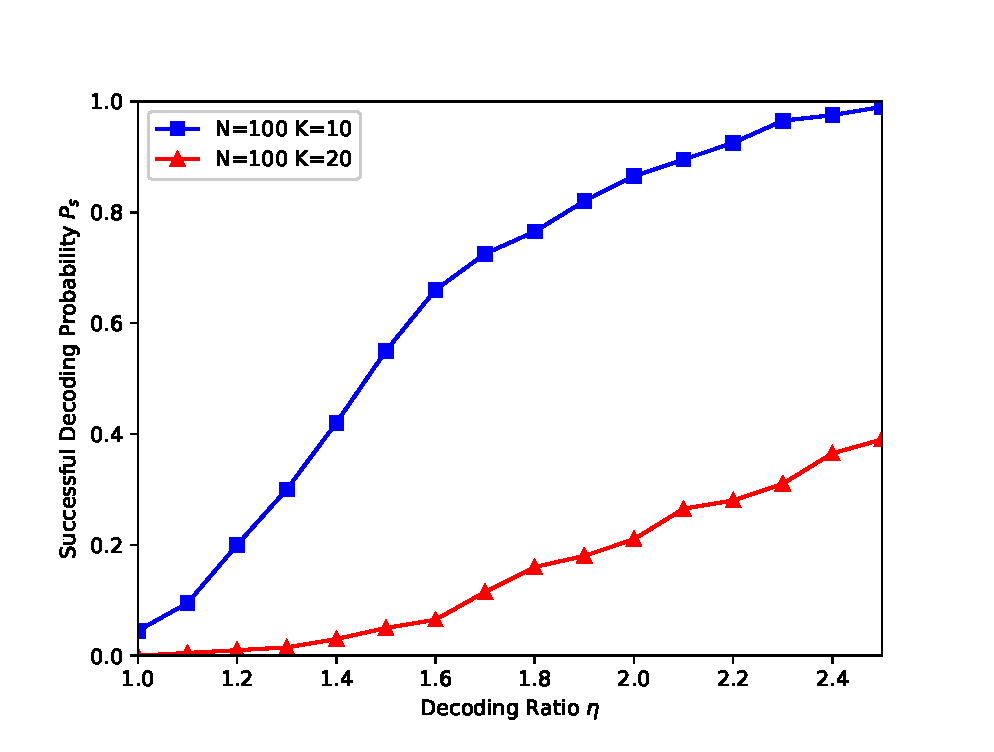
\includegraphics[width=0.9\columnwidth]{ratiovsprob.eps}
  \caption{Successfull decoding probability $P_s$ for different values of $N$, $K$ and decoding ratio $\nu$.}
  \label{fig:ratiovsprob}
\end{figure}

\section{Conclusions And Future Work}
\label{sec:conclusions}

\bibliographystyle{IEEEtran}
\bibliography{bibliography}

\end{document}
